\subsection{Эмпирическая функция распределения}
	\begin{figure}[H]
		\centering
		\begin{tabular}{ccc}
			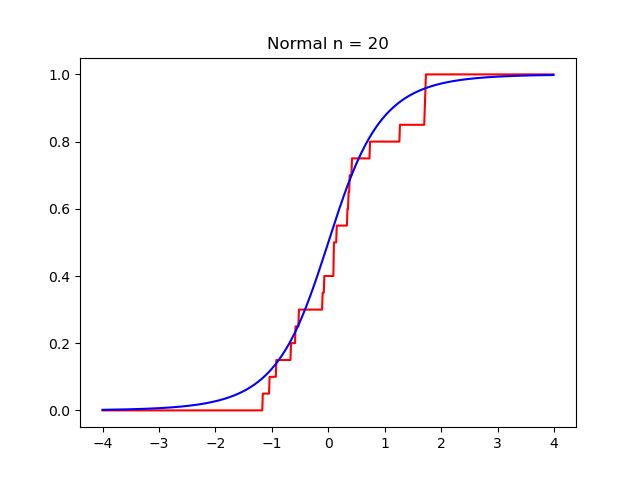
\includegraphics[width=55mm, height =0.25\textheight]{pics/emp_n_20.png}
			&
			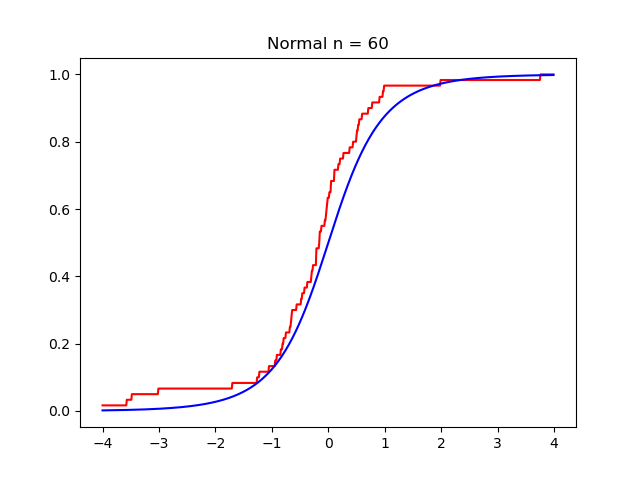
\includegraphics[width=55mm, height =0.25\textheight]{pics/emp_n_60.png}
			&
			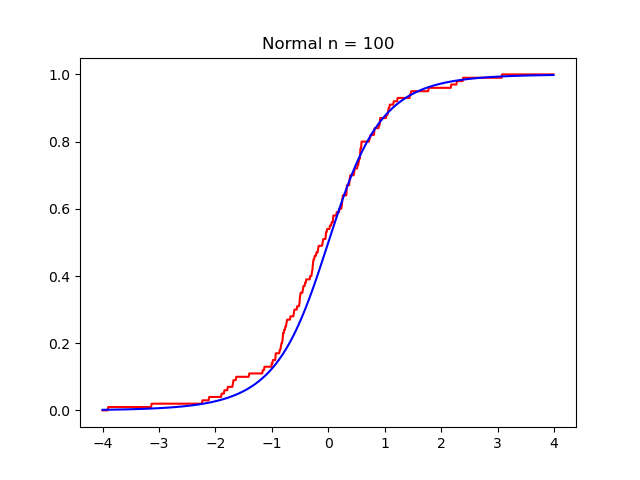
\includegraphics[width=55mm, height =0.25\textheight]{pics/emp_n_100.png}
		\end{tabular}
		\caption{Нормальное распределение}
		\label{fig:normal}
	\end{figure}

	\begin{figure}[H]
		\centering
		\begin{tabular}{ccc}
			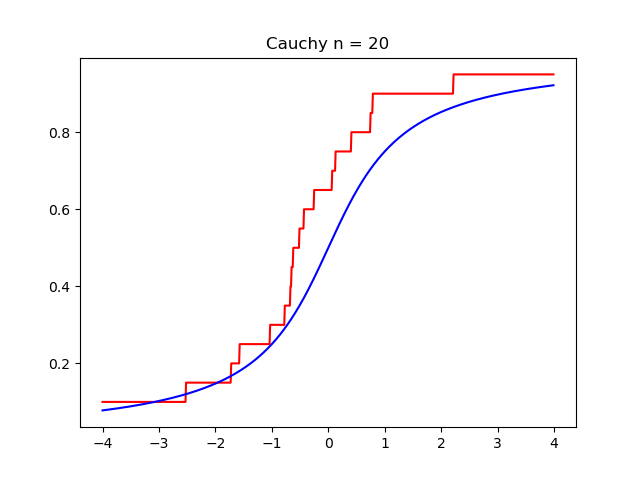
\includegraphics[width=55mm, height =0.25\textheight]{pics/emp_c_20.png}
			&
			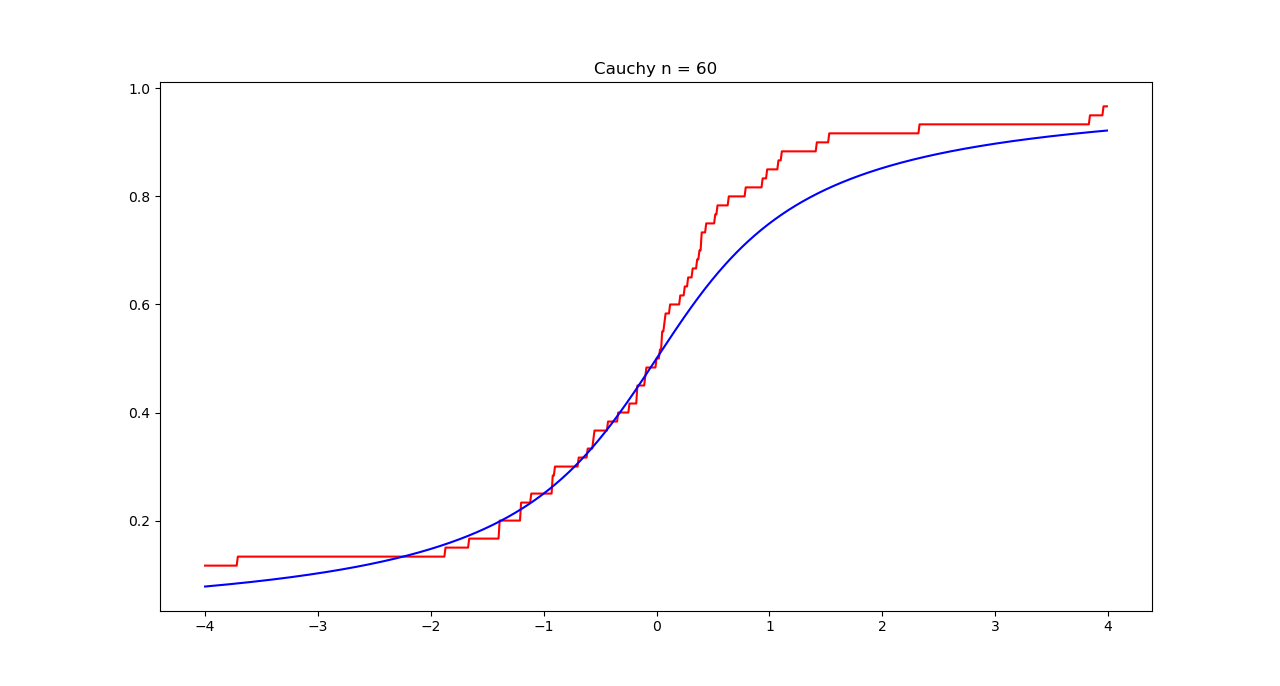
\includegraphics[width=55mm, height =0.25\textheight]{pics/emp_c_60.png}
			&
			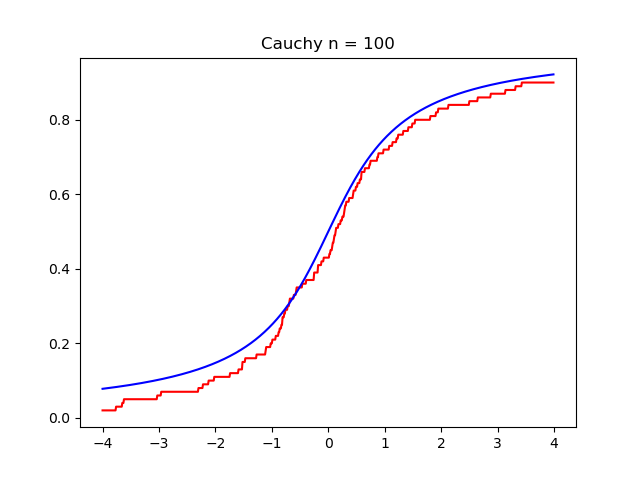
\includegraphics[width=55mm, height =0.25\textheight]{pics/emp_c_100.png}
		\end{tabular}
		\caption{Распределение Коши}
		\label{fig:cauchy}
	\end{figure}
	

	\begin{figure}[H]
		\centering
		\begin{tabular}{ccc}
			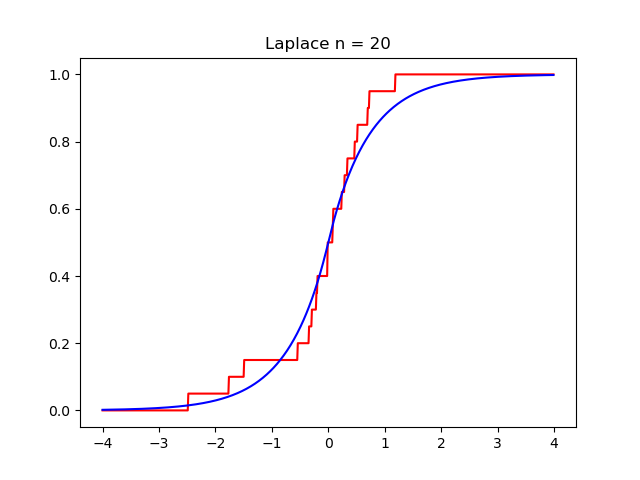
\includegraphics[width=55mm, height =0.25\textheight]{pics/emp_l_20.png}
			&
			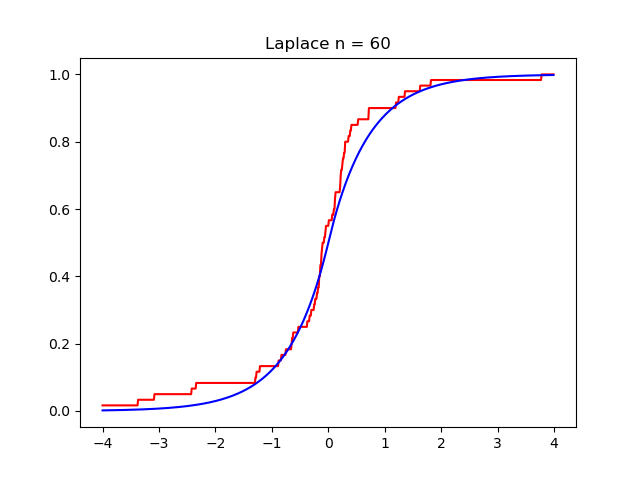
\includegraphics[width=55mm, height =0.25\textheight]{pics/emp_l_60.png}
			&
			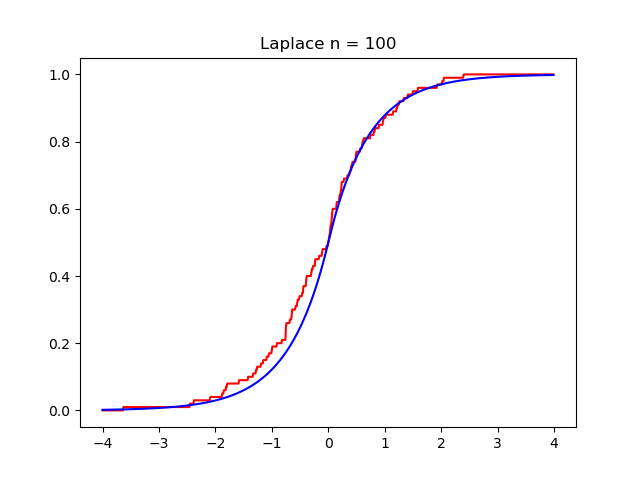
\includegraphics[width=55mm, height =0.25\textheight]{pics/emp_l_100.png}
		\end{tabular}
		\caption{Распределение Лапласа}
		\label{fig:laplace}
	\end{figure}


	\begin{figure}[H]
		\centering
		\begin{tabular}{ccc}
			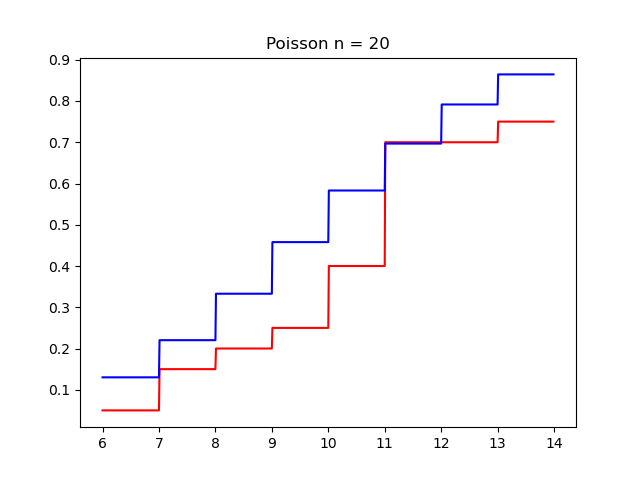
\includegraphics[width=55mm, height =0.25\textheight]{pics/emp_p_20.png}
			&
			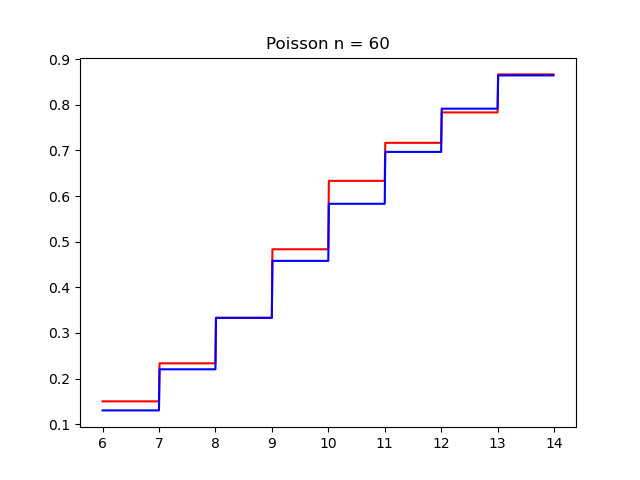
\includegraphics[width=55mm, height =0.25\textheight]{pics/emp_p_60.png}
			&
			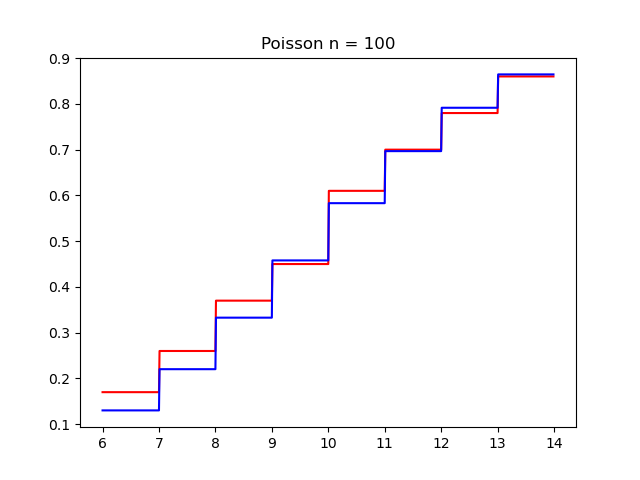
\includegraphics[width=55mm, height =0.25\textheight]{pics/emp_p_100.png}
		\end{tabular}
		\caption{Распределение Пуассона}
		\label{fig:poisson}
	\end{figure}


	\begin{figure}[H]
		\centering
		\begin{tabular}{ccc}
			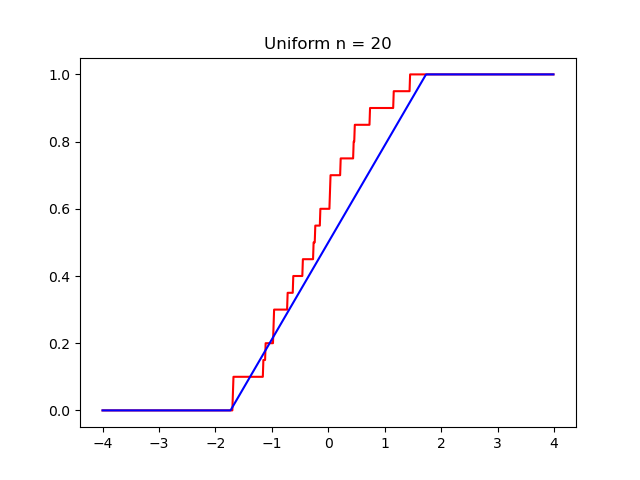
\includegraphics[width=55mm, height =0.25\textheight]{pics/emp_u_20.png}
			&
			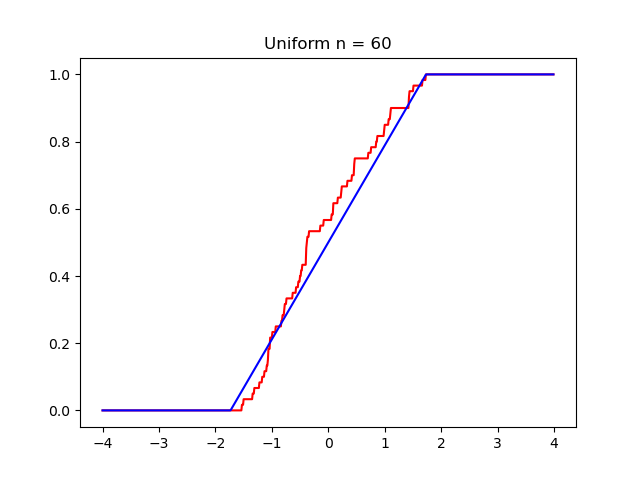
\includegraphics[width=55mm, height =0.25\textheight]{pics/emp_u_60.png}
			&
			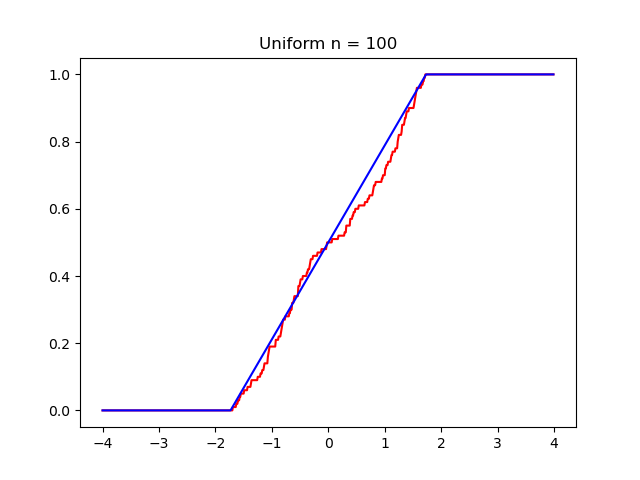
\includegraphics[width=55mm, height =0.25\textheight]{pics/emp_u_100.png}
		\end{tabular}
		\caption{Равномерное распределение}
		\label{fig:uniform}
	\end{figure}

\subsection{Ядерные оценки плотности распределения}
	\begin{figure}[H]
		\centering
			\begin{tabular}{ccc}
			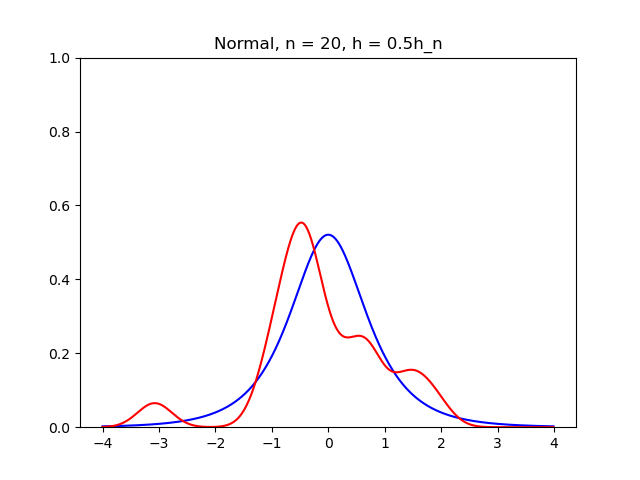
\includegraphics[width=55mm, height =0.25\textheight]{pics/ker_n_20_1.png}
			&
			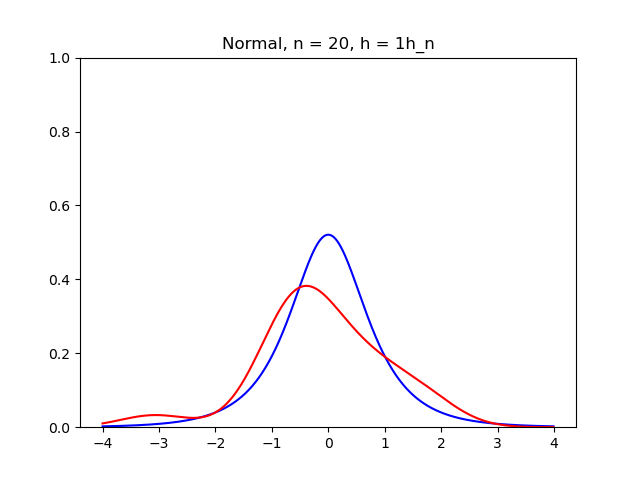
\includegraphics[width=55mm, height =0.25\textheight]{pics/ker_n_20_2.png}
			&
			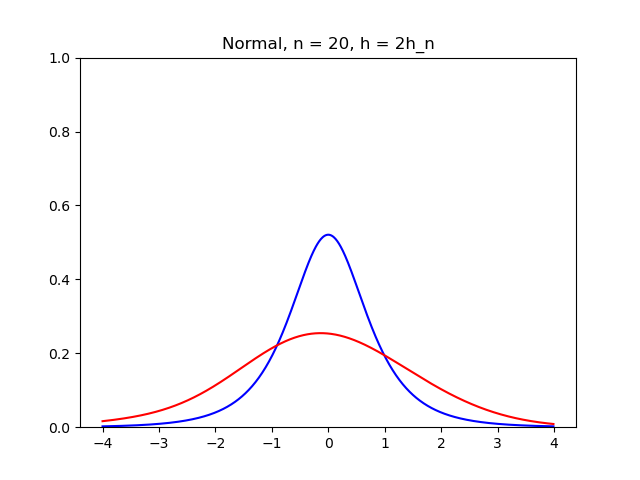
\includegraphics[width=55mm, height =0.25\textheight]{pics/ker_n_20_3.png}
			\end{tabular}
		\caption{Нормальное распределение, $n = 20$}
		\label{fig:normal}
	\end{figure}

	\begin{figure}[H]
		\centering
		\begin{tabular}{ccc}
			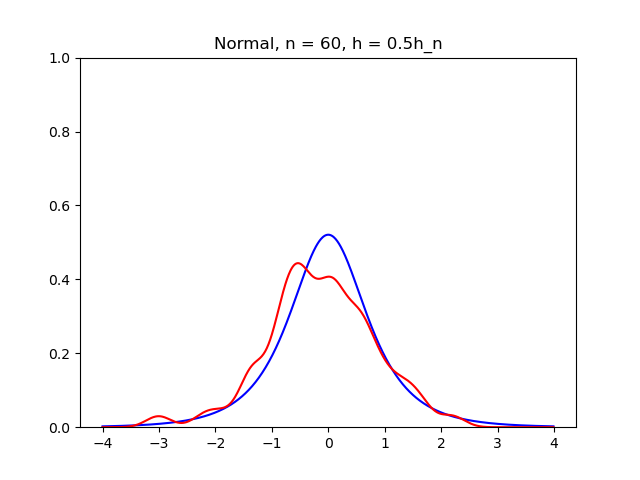
\includegraphics[width=55mm, height =0.25\textheight]{pics/ker_n_60_1.png}
			&
			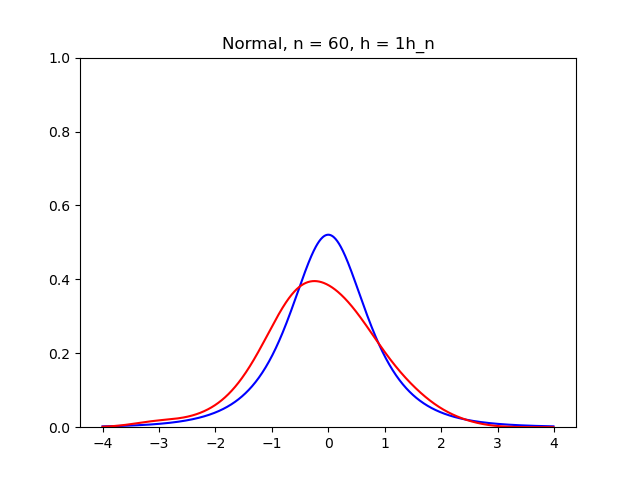
\includegraphics[width=55mm, height =0.25\textheight]{pics/ker_n_60_2.png}
			&
			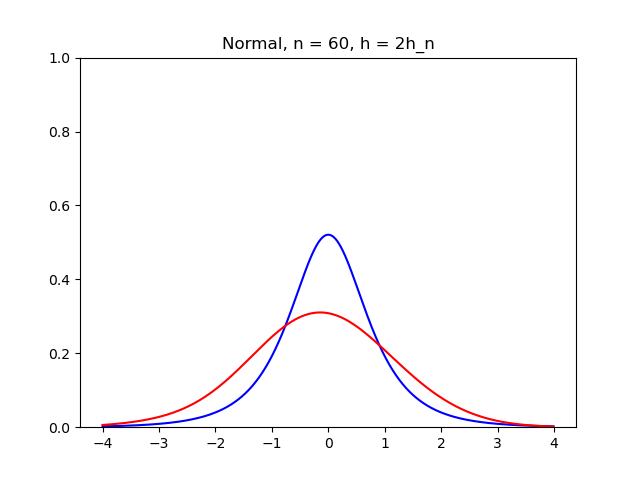
\includegraphics[width=55mm, height =0.25\textheight]{pics/ker_n_60_3.png}
		\end{tabular}
		\caption{Нормальное распределение, $n = 60$}
		\label{fig:normal}
	\end{figure}

	\begin{figure}[H]
		\centering
		\begin{tabular}{ccc}
			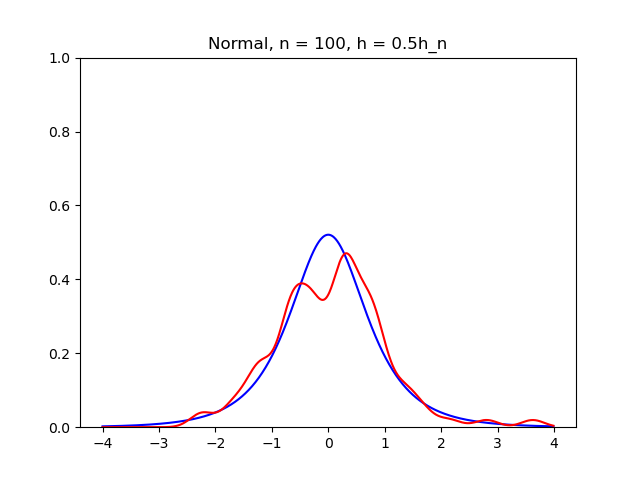
\includegraphics[width=55mm, height =0.25\textheight]{pics/ker_n_100_1.png}
			&
			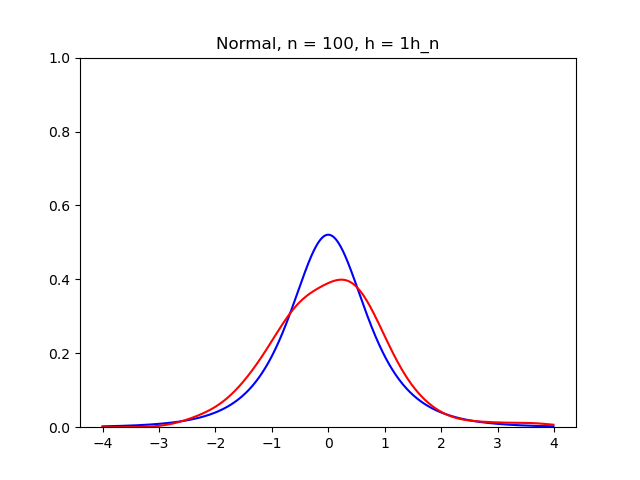
\includegraphics[width=55mm, height =0.25\textheight]{pics/ker_n_100_2.png}
			&
			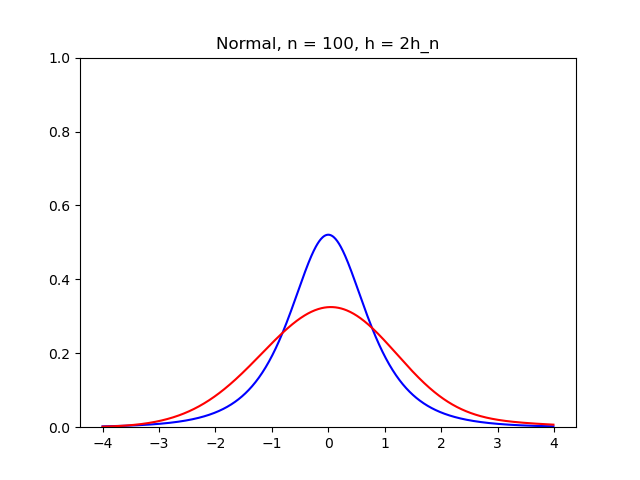
\includegraphics[width=55mm, height =0.25\textheight]{pics/ker_n_100_3.png}
		\end{tabular}
		\caption{Нормальное распределение, $n = 100$}
		\label{fig:normal}
	\end{figure}
	
	\begin{figure}[H]
		\centering
		\begin{tabular}{ccc}
			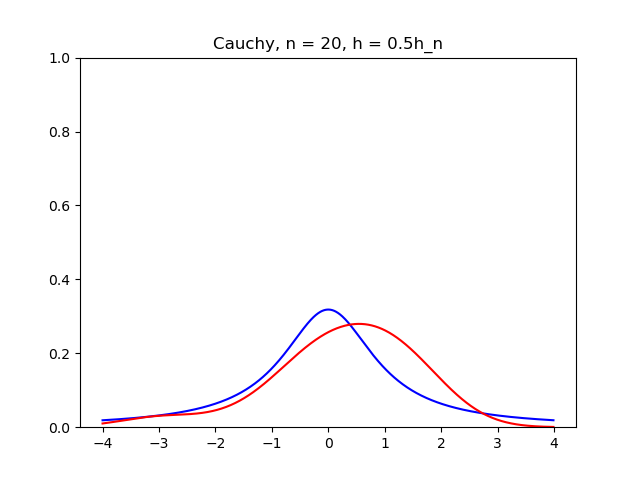
\includegraphics[width=55mm, height =0.25\textheight]{pics/ker_c_20_1.png}
			&
			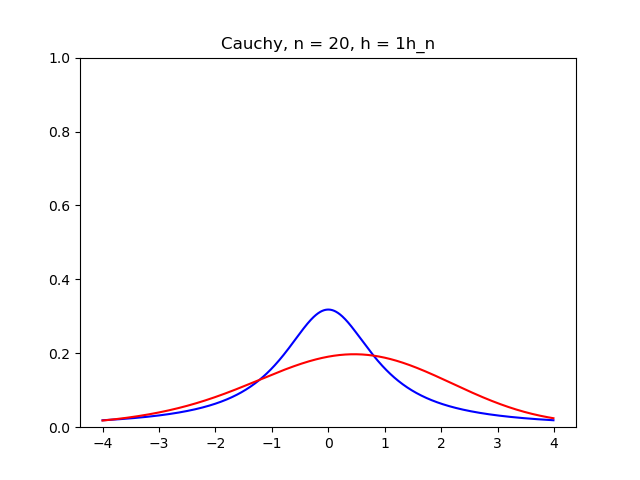
\includegraphics[width=55mm, height =0.25\textheight]{pics/ker_c_20_2.png}
			&
			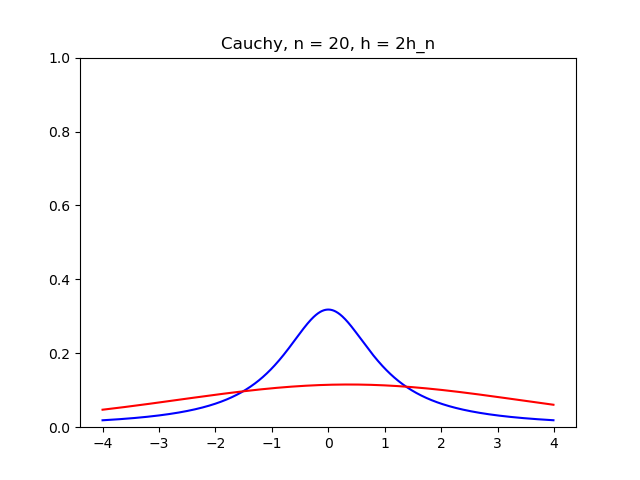
\includegraphics[width=55mm, height =0.25\textheight]{pics/ker_c_20_3.png}
		\end{tabular}
		\caption{Распределение Коши, $n = 20$}
		\label{fig:cauchy}
	\end{figure}

	\begin{figure}[H]
		\centering
		\begin{tabular}{ccc}
			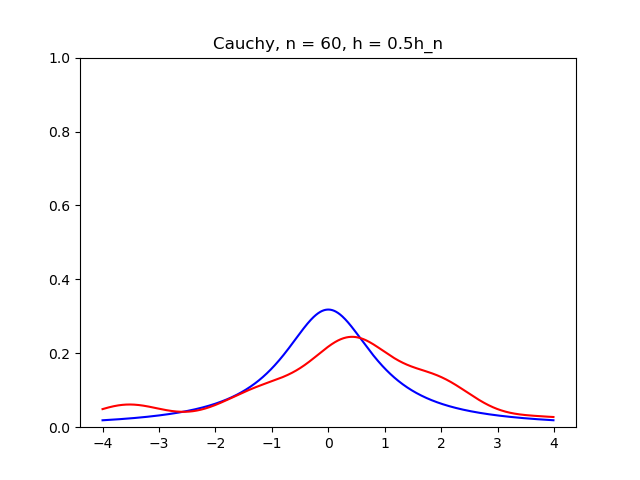
\includegraphics[width=55mm, height =0.25\textheight]{pics/ker_c_60_1.png}
			&
			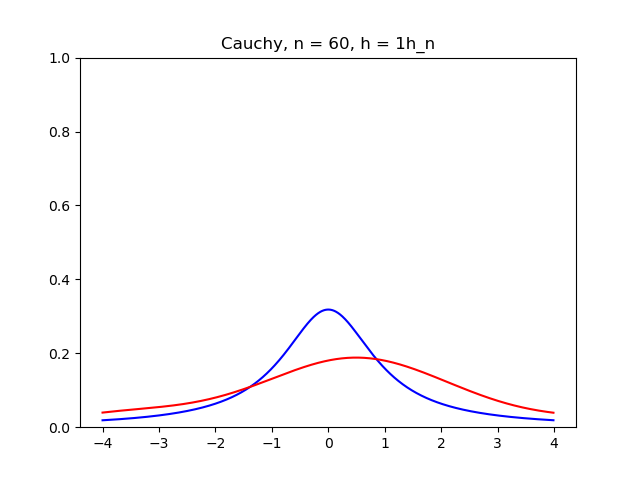
\includegraphics[width=55mm, height =0.25\textheight]{pics/ker_c_60_2.png}
			&
			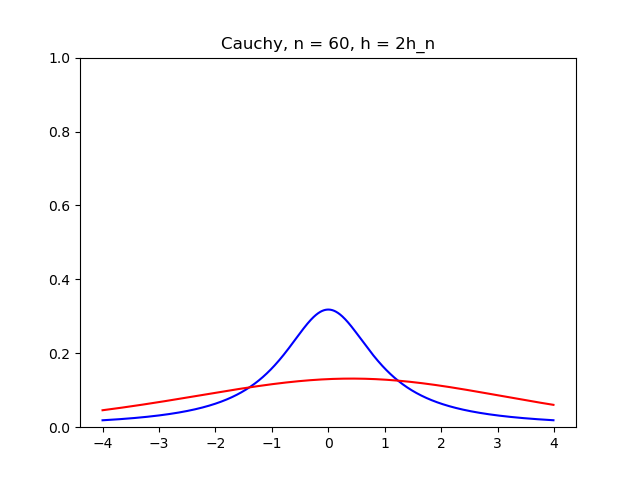
\includegraphics[width=55mm, height =0.25\textheight]{pics/ker_c_60_3.png}
		\end{tabular}
		\caption{Распределение Коши, $n = 60$}
		\label{fig:cauchy}
	\end{figure}

	\begin{figure}[H]
		\centering
		\begin{tabular}{ccc}
			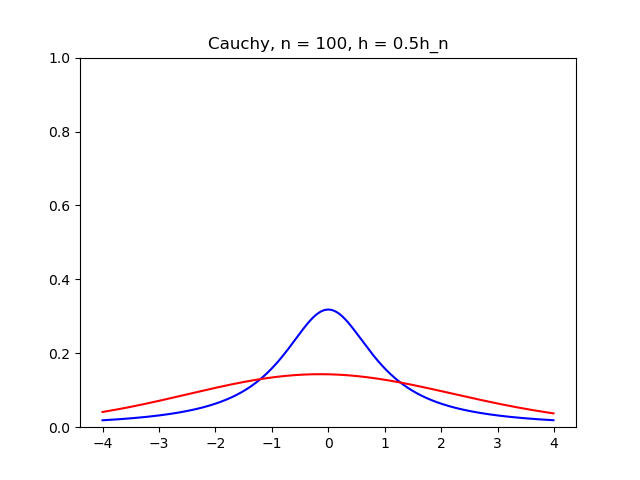
\includegraphics[width=55mm, height =0.25\textheight]{pics/ker_c_100_1.png}
			&
			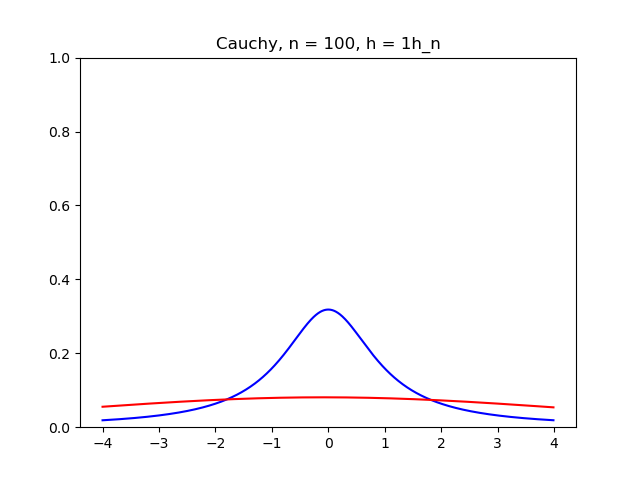
\includegraphics[width=55mm, height =0.25\textheight]{pics/ker_c_100_2.png}
			&
			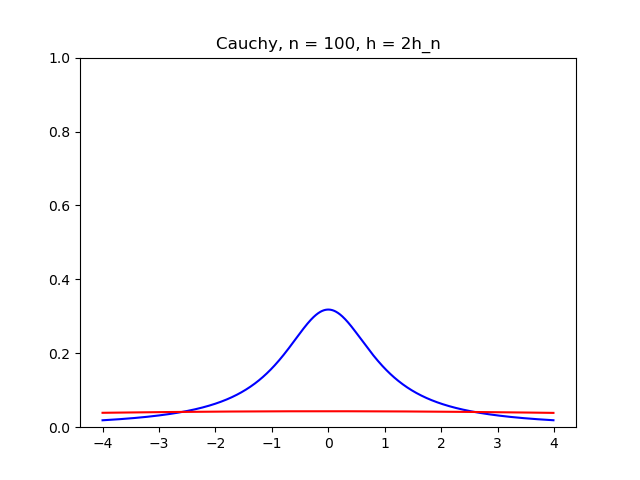
\includegraphics[width=55mm, height =0.25\textheight]{pics/ker_c_100_3.png}
		\end{tabular}
		\caption{Распределение Коши, $n = 100$}
		\label{fig:cauchy}
	\end{figure}
	
	
	\begin{figure}[H]
		\centering
		\begin{tabular}{ccc}
			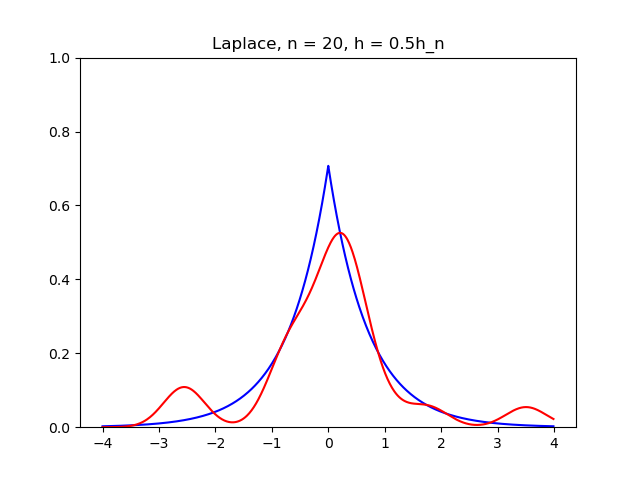
\includegraphics[width=55mm, height =0.25\textheight]{pics/ker_l_20_1.png}
			&
			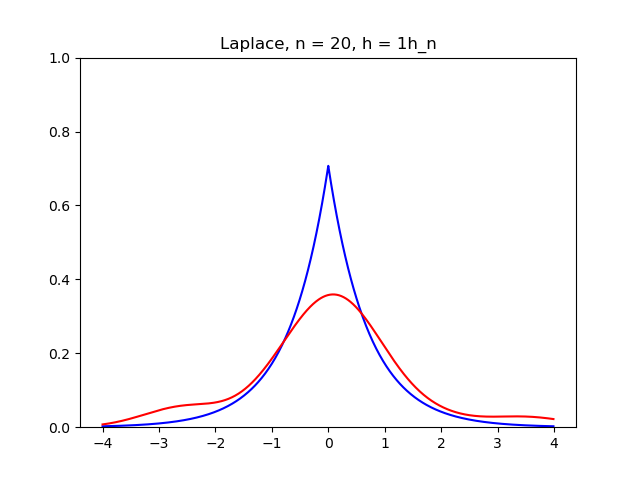
\includegraphics[width=55mm, height =0.25\textheight]{pics/ker_l_20_2.png}
			&
			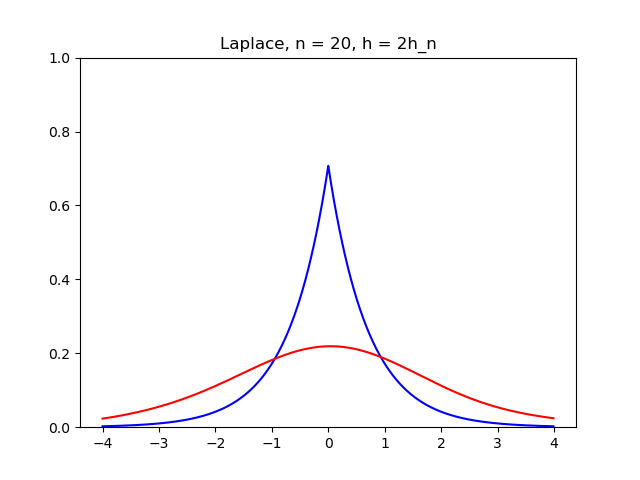
\includegraphics[width=55mm, height =0.25\textheight]{pics/ker_l_20_3.png}
		\end{tabular}
		\caption{Распределение Лапласа, $n = 20$}
		\label{fig:laplace}
	\end{figure}

	\begin{figure}[H]
		\centering
		\begin{tabular}{ccc}
			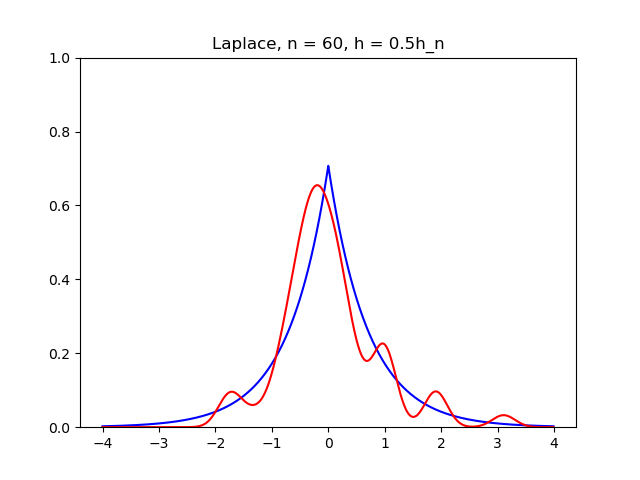
\includegraphics[width=55mm, height =0.25\textheight]{pics/ker_l_60_1.png}
			&
			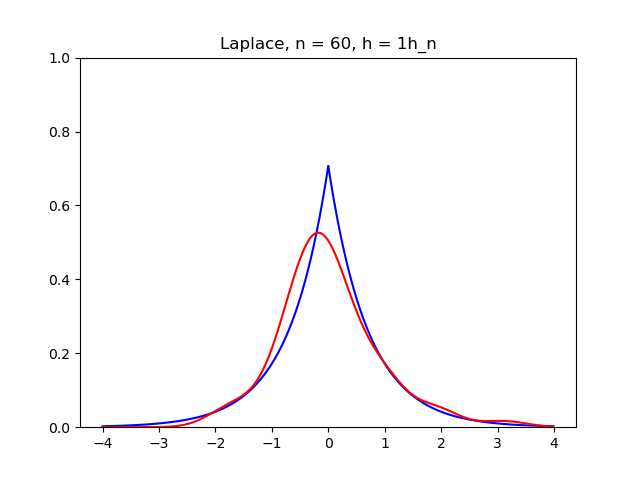
\includegraphics[width=55mm, height =0.25\textheight]{pics/ker_l_60_2.png}
			&
			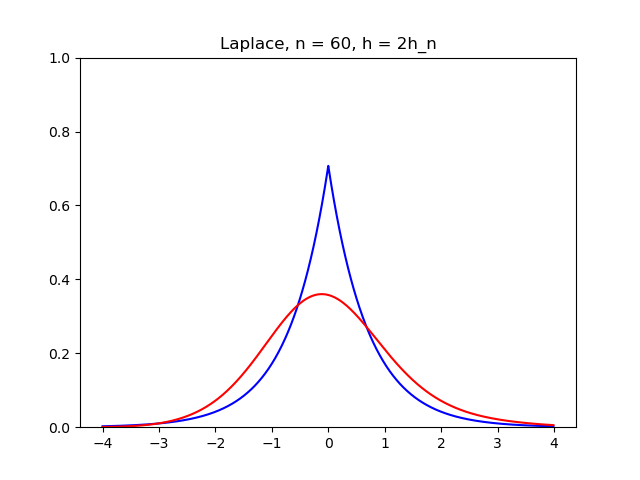
\includegraphics[width=55mm, height =0.25\textheight]{pics/ker_l_60_3.png}
		\end{tabular}
		\caption{Распределение Лапласа, $n = 60$}
		\label{fig:laplace}
	\end{figure}

	\begin{figure}[H]
		\centering
		\begin{tabular}{ccc}
			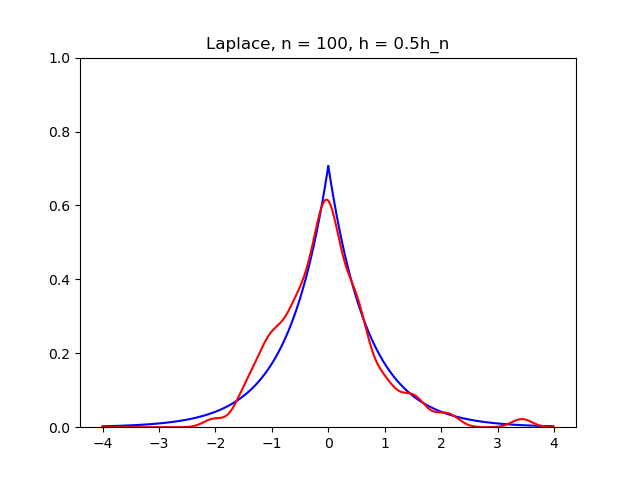
\includegraphics[width=55mm, height =0.25\textheight]{pics/ker_l_100_1.png}
			&
			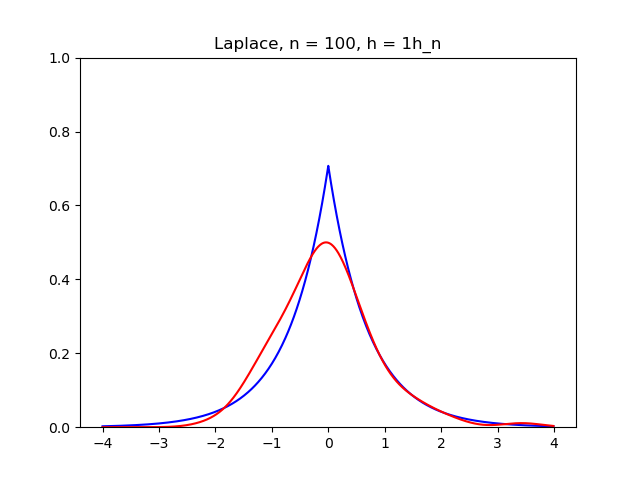
\includegraphics[width=55mm, height =0.25\textheight]{pics/ker_l_100_2.png}
			&
			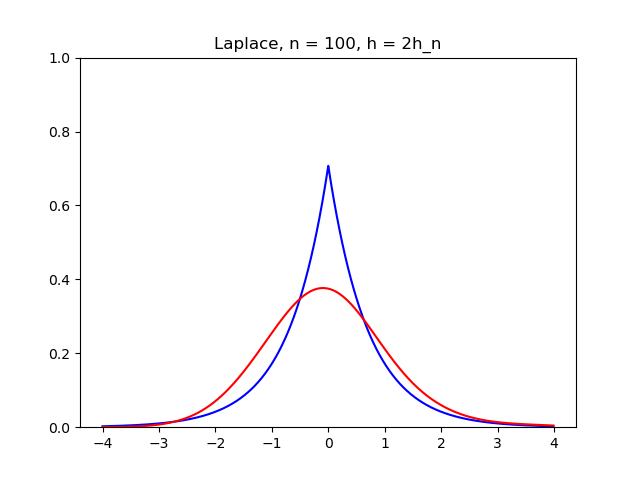
\includegraphics[width=55mm, height =0.25\textheight]{pics/ker_l_100_3.png}
		\end{tabular}
		\caption{Распределение Лапласа, $n = 100$}
		\label{fig:laplace}
	\end{figure}
	
	
	\begin{figure}[H]
		\centering
		\begin{tabular}{ccc}
			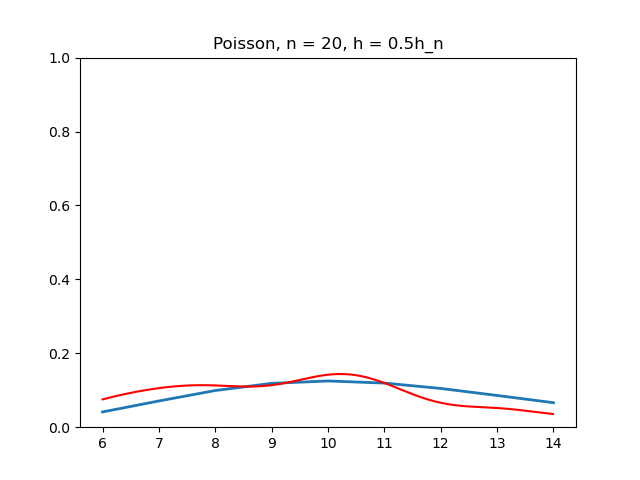
\includegraphics[width=55mm, height =0.25\textheight]{pics/ker_p_20_1.png}
			&
			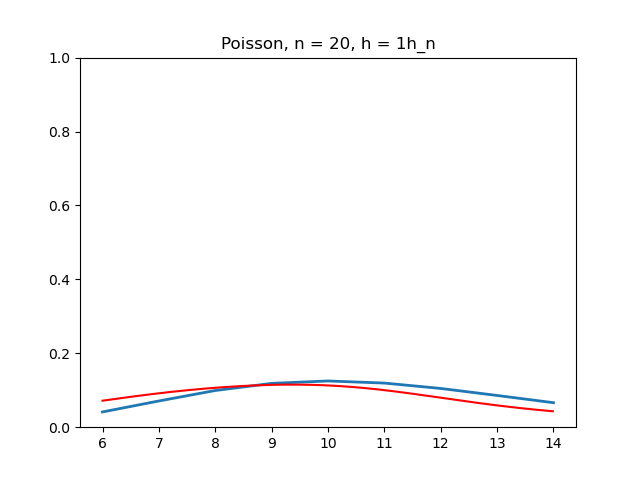
\includegraphics[width=55mm, height =0.25\textheight]{pics/ker_p_20_2.png}
			&
			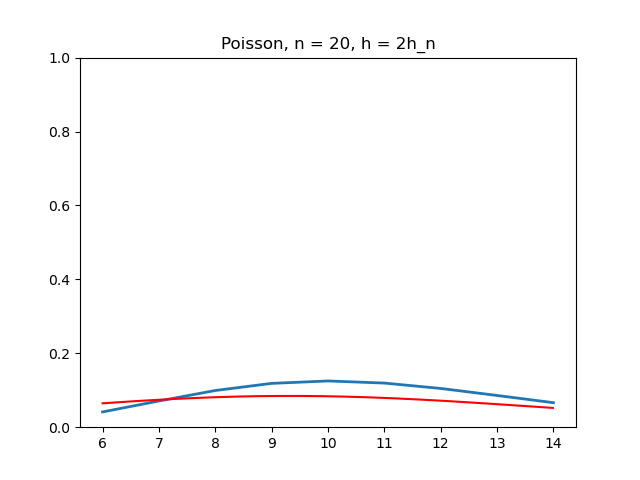
\includegraphics[width=55mm, height =0.25\textheight]{pics/ker_p_20_3.png}
		\end{tabular}
		\caption{Распределение Пуассона, $n = 20$}
		\label{fig:poisson}
	\end{figure}

	\begin{figure}[H]
		\centering
		\begin{tabular}{ccc}
			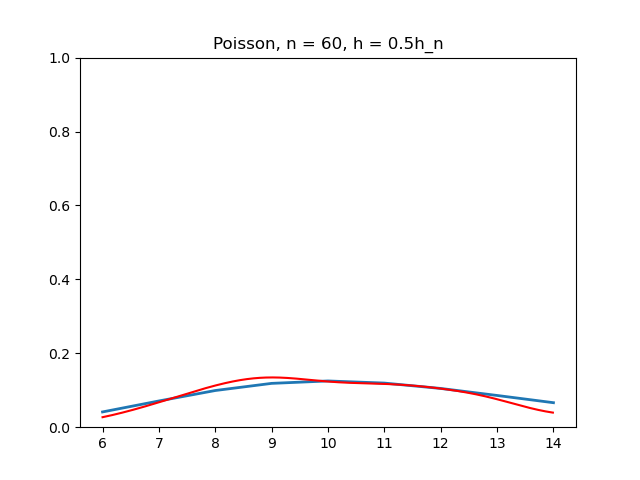
\includegraphics[width=55mm, height =0.25\textheight]{pics/ker_p_60_1.png}
			&
			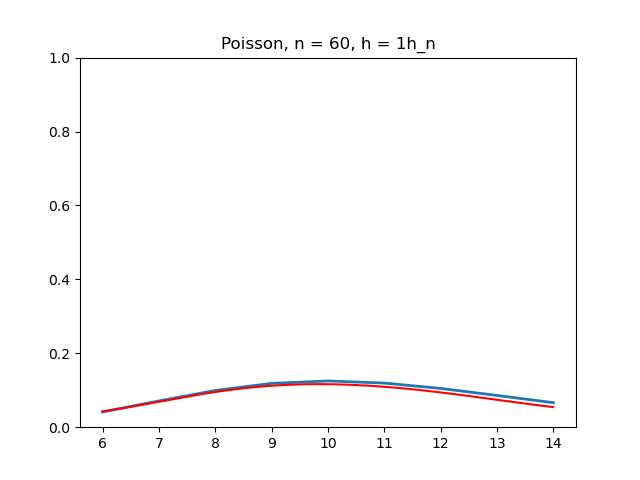
\includegraphics[width=55mm, height =0.25\textheight]{pics/ker_p_60_2.png}
			&
			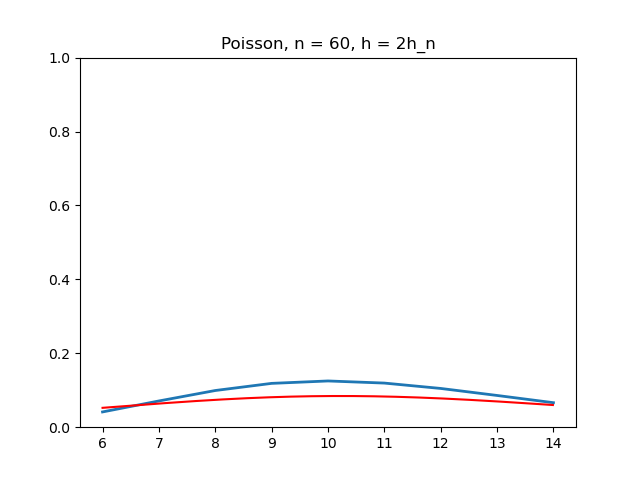
\includegraphics[width=55mm, height =0.25\textheight]{pics/ker_p_60_3.png}
		\end{tabular}
		\caption{Распределение Пуассона, $n = 60$}
		\label{fig:poisson}
	\end{figure}

	\begin{figure}[H]
		\centering
		\begin{tabular}{ccc}
			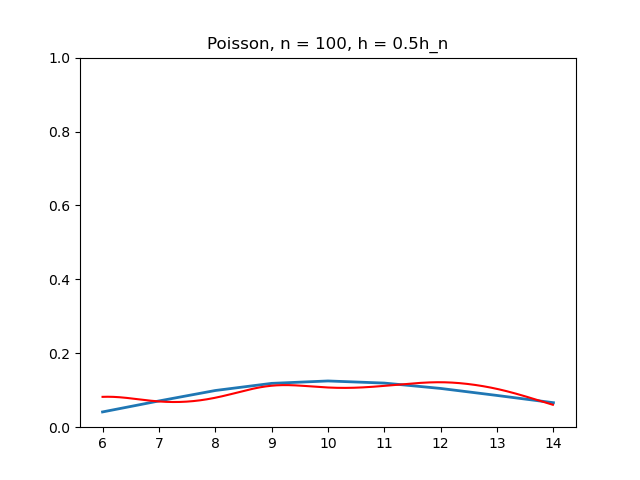
\includegraphics[width=55mm, height =0.25\textheight]{pics/ker_p_100_1.png}
			&
			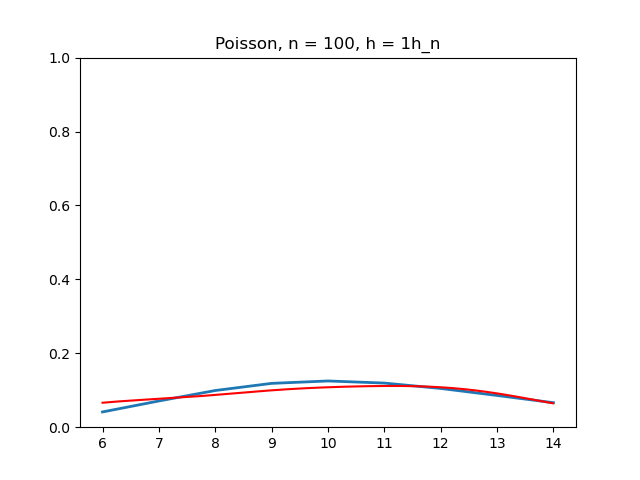
\includegraphics[width=55mm, height =0.25\textheight]{pics/ker_p_100_2.png}
			&
			\includegraphics[width=55mm, height =0.25\textheight]{pics/ker_p_100_3.png}
		\end{tabular}
		\caption{Распределение Пуассона, $n = 100$}
		\label{fig:poisson}
	\end{figure}
	
	
	\begin{figure}[H]
		\centering
		\begin{tabular}{ccc}
			\includegraphics[width=55mm, height =0.25\textheight]{pics/ker_u_20_1.png}
			&
			\includegraphics[width=55mm, height =0.25\textheight]{pics/ker_u_20_2.png}
			&
			\includegraphics[width=55mm, height =0.25\textheight]{pics/ker_u_20_3.png}
		\end{tabular}
		\caption{Равномерное распределение, $n = 20$}
		\label{fig:uniform}
	\end{figure}


	\begin{figure}[H]
	\centering
	\begin{tabular}{ccc}
		\includegraphics[width=55mm, height =0.25\textheight]{pics/ker_u_60_1.png}
		&
		\includegraphics[width=55mm, height =0.25\textheight]{pics/ker_u_60_2.png}
		&
		\includegraphics[width=55mm, height =0.25\textheight]{pics/ker_u_60_3.png}
	\end{tabular}
	\caption{Равномерное распределение, $n = 60$}
	\label{fig:uniform}
	\end{figure}

	\begin{figure}[H]
	\centering
	\begin{tabular}{ccc}
		\includegraphics[width=55mm, height =0.25\textheight]{pics/ker_u_100_1.png}
		&
		\includegraphics[width=55mm, height =0.25\textheight]{pics/ker_u_100_2.png}
		&
		\includegraphics[width=55mm, height =0.25\textheight]{pics/ker_u_100_3.png}
	\end{tabular}
	\caption{Равномерное распределение, $n = 100$}
	\label{fig:uniform}
	\end{figure}
	
